\documentclass[border=10pt]{standalone}
\usepackage{tikz}

\begin{document}
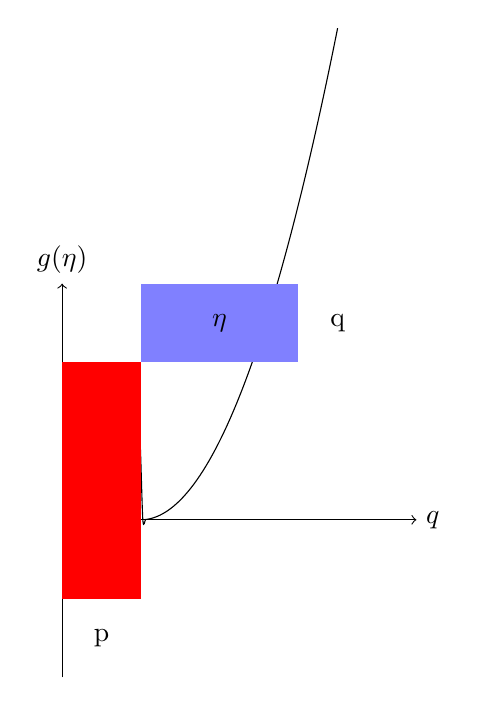
\begin{tikzpicture}
    % Axes
    \draw[->] (0,0) -- (4.5,0) node[right] {$q$};
    \draw[->] (0,-2) -- (0,3) node[above] {$g(\eta)$};

    % Plot
    \draw[domain=0:3.5,smooth,samples=100] plot ({\x}, {\x<1 ? 1 : (\x-1)^2});
    
    % Fill areas
    \fill[red] (0,-1) rectangle (1,2);
    \fill[blue!50] (1,2) rectangle (3,3);

    % Labels
    \node at (0.5,-1.5) {p};
    \node at (2,2.5) {$\eta$};
    \node at (3.5,2.5) {q};
\end{tikzpicture}
\end{document}